\documentclass[11pt,a4paper]{report}
\usepackage{marvosym}

\assignment{3}
\group{...}
\students{..........}{..........}

\begin{document}

\maketitle

Answer to the questions by by adding text in the boxes. You may answer in either \textbf{French or English}. Do not modify anything else in the template.  The size of the boxes indicate the place you \textit{can} use, but you \textit{need not} use all of it (it is not an indication of any expected length of answer). Be as concise as possible! A good short answer is better than a lot of nonsense ;-)
\bigskip

\section{Alpha-Beta search (5~pts)}

\textit{The following figure assigns a unique letter to each node, and a unique number to each branch. Use it to answer the following questions.}
\begin{center}
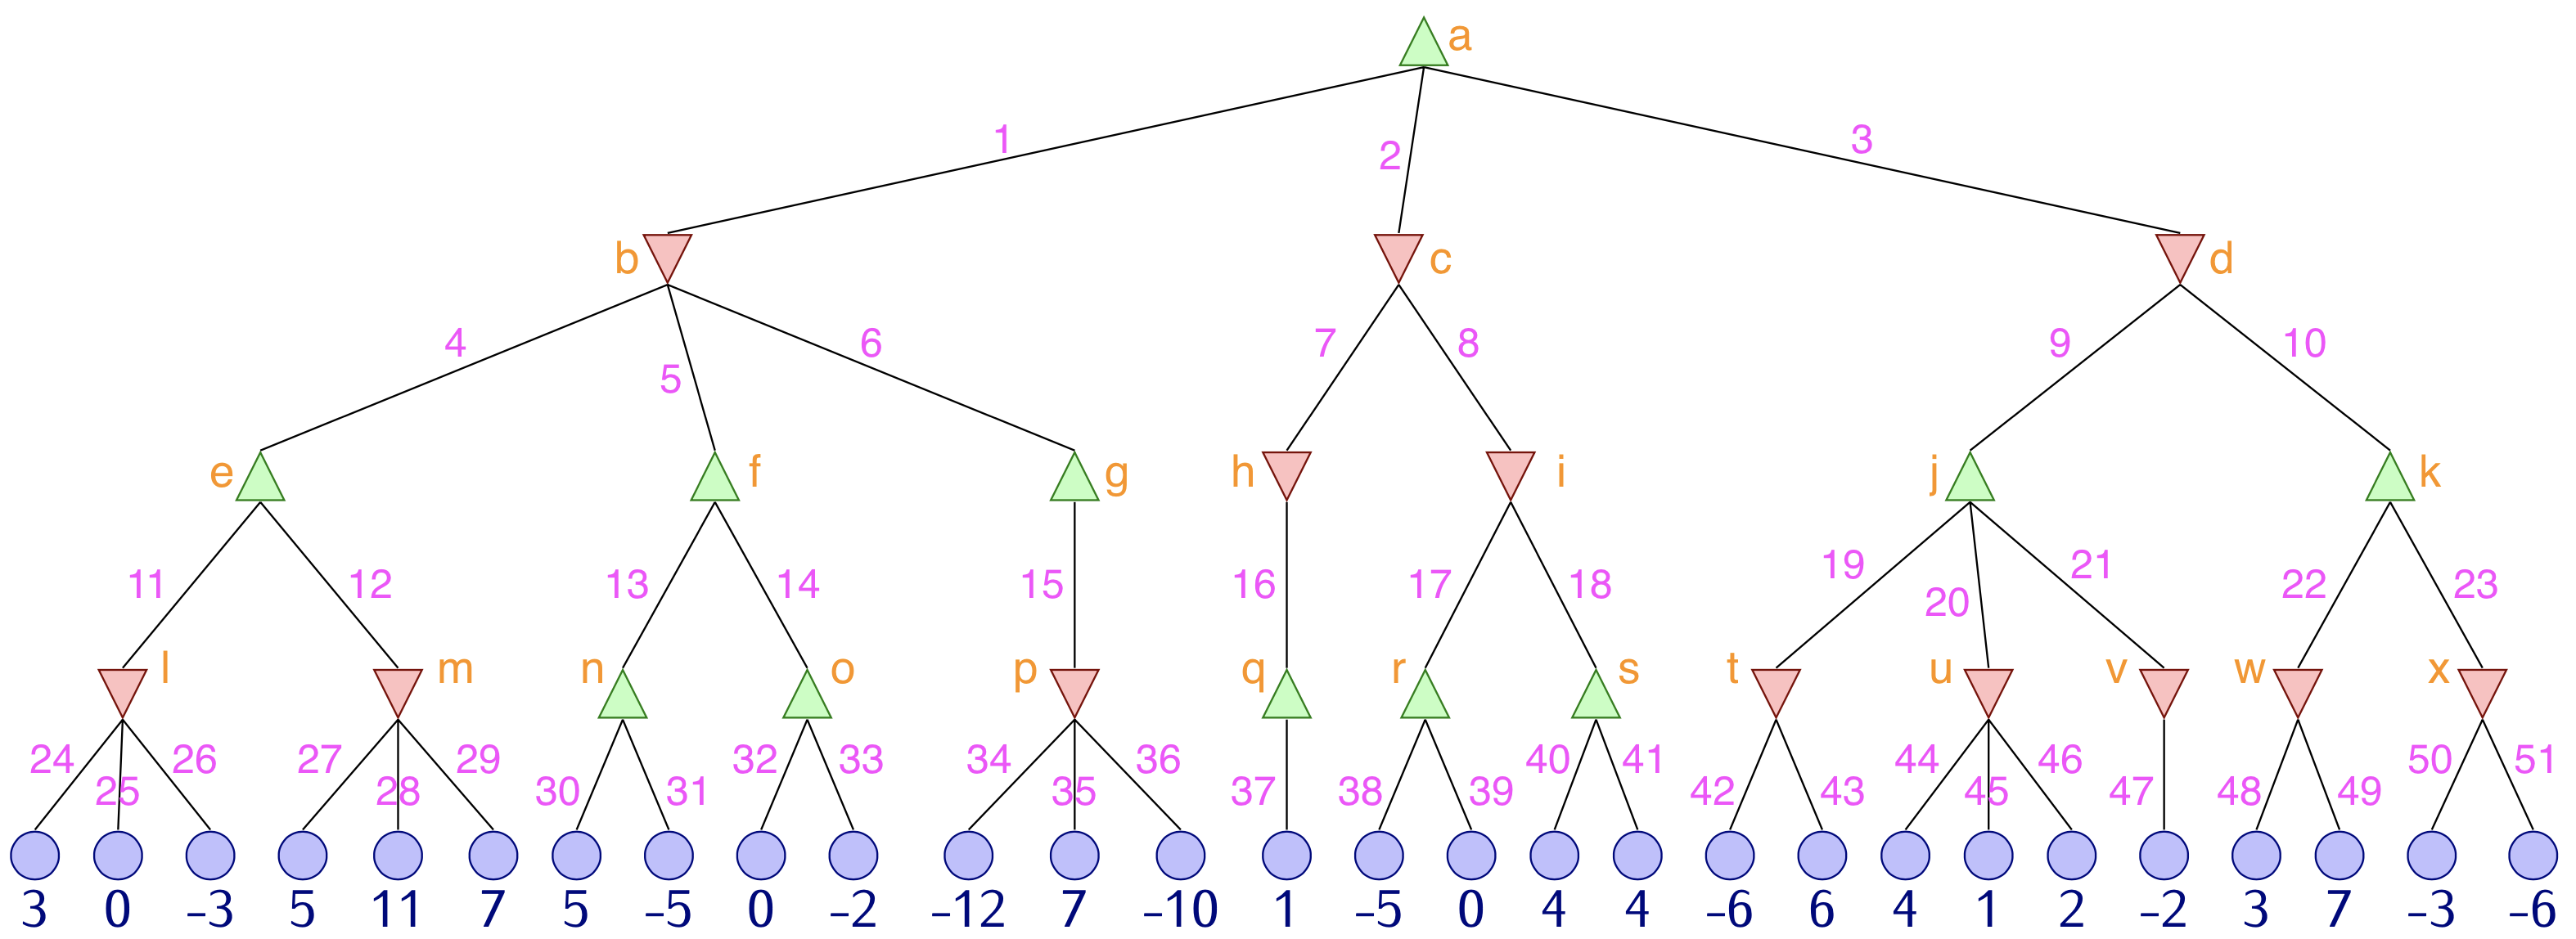
\includegraphics[scale=.3]{minimax_labelled.png}
\end{center}


\begin{enumerate}
\item Perform the MiniMax algorithm on the following tree, i.e.
      put a value to each node. What move should the root player do? \textbf{(1~pt)}
      
      \textit{Assign a numerical value to each node, and indicate the move (i.e.\! 1, 2, or 3) to perform:}
\end{enumerate}
      \begin{answers}[3cm]
      \begin{multicols}{5}
      \textbf{a: } %TODO Insert your answer here
      
      \textbf{b: } %TODO Insert your answer here
      
      \textbf{c: } %TODO etc.
      
      \textbf{d: }
      
      \textbf{e: }
      
      \textbf{f: }
      
      \textbf{g: }
      
      \textbf{h: }
      
      \textbf{i: }
      
      \textbf{j: }
      
      \textbf{k: }
      
      \textbf{l: }
      
      \textbf{m: }
      
      \textbf{n: }
      
      \textbf{o: }
      
      \textbf{p: }
      
      \textbf{q: }
      
      \textbf{r: }
      
      \textbf{s: }
      
      \textbf{t: }
      
      \textbf{u: }
      
      \textbf{v: }
      
      \textbf{w: }
      
      \textbf{x: }
      
      \textbf{Move: } %TODO Insert 1, 2 or 3 here
      \end{multicols}
	  \end{answers}



\begin{enumerate}
\item[2.] Perform the Alpha-Beta algorithm on the same tree.
      At each non terminal node, put the successive values of $\alpha$ and
      $\beta$. Cross out the arcs reaching non visited nodes. Assume a
      left-to-right node expansion. \textbf{(1~pt)}
      
      \textit{Indicate the successive $\alpha$ and $\beta$ values of each node in the table below. Separate successive values by a comma (,). Indicate at the bottom the identifiers of the branches that are cut (in increasing order, separated by a comma) (indicate only the branches where the cuts happen, i.e.\!} don't \textit{indicate the branches that are below a cut).}
\end{enumerate}

\begin{answers}[8cm]
      \begin{multicols}{2}
      \begin{tabular}{ccc}
      Node & $\alpha$ values & $\beta$ values\\
      \hline
      \textbf{a} &  &  \\ %TODO Insert your answer in the table (example: \textbf{a} & 1, 3, 2 & 5, 4 \\)
      \textbf{b} &  &  \\
      \textbf{c} &  &  \\
      \textbf{d} &  &  \\
      \textbf{e} &  &  \\
      \textbf{f} &  &  \\
      \textbf{g} &  &  \\
      \textbf{h} &  &  \\
      \textbf{i} &  &  \\
      \textbf{j} &  &  \\
      \textbf{k} &  &  \\
      \textbf{l} &  &  \\
      \end{tabular}
      
      \begin{tabular}{ccc}
      Node & $\alpha$ values & $\beta$ values\\
      \hline
      \textbf{m} &  &  \\ %TODO Insert your answer in the table
      \textbf{n} &  &  \\
      \textbf{o} &  &  \\
      \textbf{p} &  &  \\
      \textbf{q} &  &  \\
      \textbf{r} &  &  \\
      \textbf{s} &  &  \\
      \textbf{t} &  &  \\
      \textbf{u} &  &  \\
      \textbf{v} &  &  \\
      \textbf{w} &  &  \\
      \textbf{x} &  &  \\
      \end{tabular}
      \end{multicols}
      
\textbf{Cuts:} %TODO Insert your answer here (example: 2, 4, 6, 8, 10)
\end{answers}





\begin{enumerate}
\item[3.] Do the same, assuming a right-to-left node expansion instead.  \textbf{(1~pt)}
\end{enumerate}

\begin{answers}[8cm]
      \begin{multicols}{2}
      \begin{tabular}{ccc}
      Node & $\alpha$ values & $\beta$ values\\
      \hline
      \textbf{a} &  &  \\ %TODO Insert your answer in the table (example: \textbf{a} & 1, 3, 2 & 5, 4 \\)
      \textbf{b} &  &  \\
      \textbf{c} &  &  \\
      \textbf{d} &  &  \\
      \textbf{e} &  &  \\
      \textbf{f} &  &  \\
      \textbf{g} &  &  \\
      \textbf{h} &  &  \\
      \textbf{i} &  &  \\
      \textbf{j} &  &  \\
      \textbf{k} &  &  \\
      \textbf{l} &  &  \\
      \end{tabular}
      
      \begin{tabular}{ccc}
      Node & $\alpha$ values & $\beta$ values\\
      \hline
      \textbf{m} &  &  \\ %TODO Insert your answer in the table
      \textbf{n} &  &  \\
      \textbf{o} &  &  \\
      \textbf{p} &  &  \\
      \textbf{q} &  &  \\
      \textbf{r} &  &  \\
      \textbf{s} &  &  \\
      \textbf{t} &  &  \\
      \textbf{u} &  &  \\
      \textbf{v} &  &  \\
      \textbf{w} &  &  \\
      \textbf{x} &  &  \\
      \end{tabular}
      \end{multicols}
      
\textbf{Cuts:} %TODO Insert your answer here (example: 2, 4, 6, 8, 10)
\end{answers}




\clearpage
\begin{enumerate}
\item[4.] Can the nodes be ordered in such a way that Alpha-Beta pruning can cut off
      more branches (in a left-to-right node expansion)? If no, explain why; if
      yes, give the new ordering and the resulting new pruning. \textbf{(1~pt)}
      
      \textit{Insert an image below containing the reordered tree, with successive $\alpha$/$\beta$ values indicated next to each node, and where the branches that are cut by the algorithm are crossed out. This may either be an edited version of \texttt{minimax.png} (using paint, gimp, etc.), a photograph of a drawing you made by hand, etc. In any case, the image must be \textbf{clear} in order to be graded.}
\end{enumerate}

\begin{answers}[8cm]
%TODO Insert the path to your image between the {}. 
% Possibly adjust the scale parameter so your image fits in the box.
%\includegraphics[scale=.3]{...}
\end{answers}




\begin{enumerate}
\item[5.] How does Alpha-Beta need to be modified for games with more than two players? \textbf{(1~pt)}
\end{enumerate}

\begin{answers}[9cm]
%TODO Insert your answer here
\end{answers}





\clearpage
\section{Fanorona (35~pts)}
\medskip

\subsection{A Basic Alpha-Beta Agent (5~pts on INGInious; nothing to report)}
\medskip


\subsection{Evaluation function (5~pts)}

\begin{enumerate}
\item[5.] What are the weak points of the evaluation functions of your basic agent? \textbf{(2~pts)}

{\it Please list your ideas using bullet points, e.g.\! something of the form:
	\begin{itemize}
	\item \textbf{Name of your idea}
	
	Possibly a short explanation describing your idea... Go straight to the point!
	\end{itemize}}
\end{enumerate}

\begin{answers}[17cm]

\begin{itemize}
\item %TODO Insert your answers here
\item
\item
\end{itemize}

\end{answers}


\clearpage
\begin{enumerate}
\item[6.] As described in the class, an evaluation function is often a linear combination of
some features. Describe new features of a state that can be interesting when evaluating a state of this game. \textbf{(2~pts)}

\textit{As for the previous question, list your ideas using bullet points.}
\end{enumerate}

\begin{answers}[20cm]

\begin{itemize}
\item %TODO Insert your answers here
\item
\item
\end{itemize}

\end{answers}



\clearpage
\begin{enumerate}
\item[7.] Describe precisely your improved evaluation function. \textbf{(1~pt)}
\end{enumerate}

\begin{answers}[20cm]
%TODO Insert your answer here
\end{answers}






\clearpage
\subsection{Successors function (4~pts)}

\begin{enumerate}
\item[8.] Give an upper bound on the maximum number of actions that can be performed in
any given state. If you can't, explain how you could estimate what is the average
number of successors and estimate it. \textbf{(1~pt)}
\end{enumerate}

\quad \textit{Put your numeric answer here (if you can't give a number, put an ``X'').}

\begin{smallanswers}
%TODO Insert your answer here
\end{smallanswers}

\quad \textit{Explain your answer below.}

\begin{answers}[8cm]
%TODO Insert your answer here
\end{answers}






\begin{enumerate}
\item[9.] What do you loose by ignoring some of the successors? \textbf{(1~pt)}
\end{enumerate}

\begin{answers}[8cm]
%TODO Insert your answer here
\end{answers}






\begin{enumerate}
\item[10.] Could reordering the successors help the performance of your agent? If so, in what order should the successors be returned in order to help Alpha-Beta
prune the search tree? \textbf{(1~pt)}
\end{enumerate}

\begin{answers}[9cm]
%TODO Insert your answer here
\end{answers}





\begin{enumerate}
\item[11.] Describe you successor function. \textbf{(1~pt)}
\end{enumerate}

\begin{answers}[9cm]
%TODO Insert your answer here
\end{answers}





\clearpage
\subsection{Cut-off function (4~pts)}


\begin{enumerate}
\item[12.] The \lstinline|cutoff| method receives an argument called
    \lstinline|depth|. Explain precisely what is called the
    \emph{depth} in the \lstinline|minimax.py| implementation. \textbf{(1~pt)}
\end{enumerate}

\begin{answers}[6cm]
%TODO Insert your answer here
\end{answers}





\begin{enumerate}
\item[13.] The \lstinline|cutoff| function is also the one responsible for identifying which states lead to the end of the game (and so possible victory or defeat). Usually, the end is obtained when one player has lost all of its pawns. However, a situation where each player has a limited number of pawns could lead to an infinite game, where each one is able to escape the other. By convention, the victory is then given to player which has the most pawns. In the implementation, this is dealt with by ending the game when 50 ``boring moves'' (i.e.\! no capture of an opponent pawn) have occurred. Why could such an approach be problematic for an Alpha-Beta agent? How could you remedy this? \textbf{(1~pt)}
\end{enumerate}

\begin{answers}[10cm]
%TODO Insert your answer here
\end{answers}





\begin{enumerate}
\item[14.] In the Fanorona contest your agent will be credited a limited time.
How do you manage that time? How can you make sure that you will never timeout?
Explain how you can use \emph{iterative deepening} to avoid timeouts. \textbf{(1~pt)}
\end{enumerate}

\begin{answers}[10cm]
%TODO Insert your answer here
\end{answers}






\begin{enumerate}
\item[15.] Describe your cut-off function. \textbf{(1~pt)}
\end{enumerate}

\begin{answers}[9cm]
%TODO Insert your answer here
\end{answers}





\clearpage
\subsection{A Smart Alpha-Beta Agent (6~pts on INGInious)}
\medskip

\subsection{Contest (6~pts on INGInious; 5~pts for report)}


\begin{enumerate}
\item[18.] Describe concisely your super tough agent. \textbf{(5~pts)}
\end{enumerate}

\begin{answers}[20cm]
%TODO Insert your answer here and in the following frame if needed
\end{answers}

\begin{answers}[23cm]
%TODO Continue your answer here
\end{answers}





\end{document}
